\begin{appendices}

%Some Table of Contents entry formatting
\addtocontents{toc}{\protect\renewcommand{\protect\cftchappresnum}{\appendixname\space}}
\addtocontents{toc}{\protect\renewcommand{\protect\cftchapnumwidth}{6em}}

%Begin individual appendices, separated as chapters

\chapter{Gradient of Hybrid NLP Lagrangian}\label{appendix:A}

Explicit expressions of the formulation are provided in this
Appendix. We note that operations involving the symbol $\nabla$ map scalars to
vectors and vectors to matrices. For example, if $f:\mathbb{R}^p\rightarrow 
\mathbb{R}$ and
$\bvec{v}:\mathbb{R}^p\rightarrow\mathbb{R}^q$, then $\nabla
f:\mathbb{R}^p\rightarrow\mathbb{R}^p$ and
$\nabla\bvec{v}:\mathbb{R}^p\rightarrow\mathbb{R}^{p\times q}$.

The Lagrangian function is used here, as presented in Eq.
(\ref{eq:langrT}):
\begin{gather}
	\mathcal{L}(\bvec{y}, \bvec{d}_g,\bvec{\lambda}) =
	U-W+\bvec{\lambda}^T\bvec{h}_g
	\label{eq:globalL}
\end{gather}

\noindent where it is also reminded that $\bvec{y} = \begin{bmatrix}
	\bvec{y}_1^T & \bvec{y}_2^T & \cdots & \bvec{y}_m^T
\end{bmatrix}^T$, $\bvec{y}_i = \begin{bmatrix}
	\bvec{q}_i & \phi_i
\end{bmatrix}^T$ and $\bvec{q}_i = \begin{bmatrix}
	\epsilon_i & \gamma_i & \kappa_i
\end{bmatrix}^T$. The number $m$ designates the \emph{total} number of
integration points in the structure.

%\subsection{Gradient of Strain Energy}
The gradient of the strain energy, $U$, is expressed as:
\begin{gather}
	\nabla U = \begin{bmatrix}
		\nabla_{\mathbf{y}}U\\ \nabla_{\mathbf{d}_g}U\\ 
		\nabla_{\mathbf{\lambda}}U
	\end{bmatrix}\nonumber
\end{gather}

\noindent The gradient with respect to the strain vector $\bvec{y}$ gives the
stress resultants at all cross-sections and has the following form for a
particular cross-section $i$:
\begin{gather}
	\nabla_{\mathbf{y}_i}U = \begin{bmatrix}
		w_iN_i\\ w_iV_i\\ w_iM_i\\ 0
	\end{bmatrix} = w_i\begin{bmatrix}
		\bvec{F}_{sec}^{(i)}\\ 0
	\end{bmatrix}
	\label{eq:straingrad}
\end{gather}

\noindent it is usually computed by numerical integration of Eqs.
(\ref{eq:fsecx}) over the cross-section height. In the case of elastic
analysis, the above vector can be computed explicitly for each cross-section,
since then $\bvec{F}_{sec}^{(i)} = \begin{bmatrix}
	EA\epsilon_i & k_sGA\gamma_i & EI\kappa_i
\end{bmatrix}^T$.

The gradients of $U$ with respect to both $\bvec{d}_g$ and $\bvec{\lambda}$
provide zero vectors:
\begin{gather}
	\nabla_{\mathbf{d}_g}U = 
	\bvec{0}\in\mathbb{R}^{3N_{nod}}\quad\text{and}\quad
	\nabla_{\mathbf{\lambda}}U = \bvec{0}\in\mathbb{R}^{s}\nonumber
\end{gather}

\noindent where $s=m + 3n_{el}$, $n_{el}$ being the number of elements.
Finally, we then get:
\begin{gather}
	\nabla U = \begin{bmatrix}
		\nabla_{\mathbf{y}}U\\ \bvec{0}\\ \bvec{0}
	\end{bmatrix}
\end{gather}

%\subsection{Gradient of Constraints}

We restate the constraints equations from Eqs.
(\ref{eq:impsd1})-(\ref{eq:impsd2}):
\begin{gather}
	\bvec{h}_g = \begin{bmatrix}
		\bvec{h}_g^A\\ \bvec{h}_g^B
	\end{bmatrix} =
	\begin{bmatrix}
		\bmat{V}_1\bvec{d}_g - \bmat{\Lambda}^T\bigg[\sum_{i=1}^n
		w_i\bmat{R}_i(\bvec{q}_i+\bvec{E}_1) - \ell\bvec{E}_1\bigg]\\
		\bvec{\phi}-\bmat{V}_2\bvec{d}_g - \bmat{T}\bvec{\kappa}
	\end{bmatrix}\nonumber
\end{gather}

\noindent For notational simplicity, we assume here only one element
in the derivations that follow. When more elements are used, their
corresponding constraint vectors are stacked in vector form as
$\bvec{h} = \begin{bmatrix}
	\ \bvec{h}_g^{1\ T}& \bvec{h}_g^{2\ T}& \cdots & \bvec{h}_g^{n_{el}\ T}
\end{bmatrix}^T$.
The gradient with respect to the strain vector
$\bvec{y}_i$ at a particular cross-section is given by:
\begin{gather}
	\nabla_{\mathbf{y}_i}\bvec{h}_g^A = \begin{bmatrix}
		\nabla_{\mathbf{q}_i}\bvec{h}_g^A &\ \dfrac{d \bvec{h}_g^A}{d\phi_i}
	\end{bmatrix} = -w_i\bmat{\Lambda}^T\begin{bmatrix}
		\bmat{R}_i &\
		\bmat{R}_i\bmat{X}[\bvec{q}_i+\bvec{E}_1]
	\end{bmatrix}\nonumber
\end{gather}

\noindent where:
\begin{gather}
	\frac{d\bmat{R}_i}{d\phi_i} = \bmat{R}_i\bmat{X}\quad\text{and}\quad
	\bmat{X} = \begin{bmatrix}
		0 & -1 & 0\\
		1 &  0 & 0\\
		0 &  0 & 0
	\end{bmatrix}\nonumber
\end{gather}

\noindent The gradient of $\bvec{h}_g^B$ with respect to strain vector
$\bvec{y}_i$, is:
\begin{gather}
	\nabla_{\mathbf{y}_i}\bvec{h}_g^B = \begin{bmatrix}
		\nabla_{\mathbf{q}_i}\bvec{h}_g^B & \dfrac{d \bvec{h}_g^B}{d\phi_i}
	\end{bmatrix} = \begin{bmatrix}
		\bvec{0} & \bvec{0} & -\bmat{T}\hat{\mathbf{E}}_i & \hat{\mathbf{E}}_i
	\end{bmatrix}\nonumber
\end{gather}

\noindent where $\hat{\mathbf{E}}_i\in\mathbb{R}^{n_q}$ is a unit vector with 
the
$i$-th component equal to one.
\noindent Collectively, we have:
\begin{gather}
	\nabla_{\mathbf{y}_i}\bvec{h}_g = \begin{bmatrix}
		-w_i\bmat{\Lambda}^T\bmat{R}_i & -w_i\bmat{\Lambda}^T
		\bmat{R}_i\bmat{X}[\bvec{q}_i+\bvec{E}_1]\\
		[\bvec{0}\quad \bvec{0}\quad -\bmat{T}\hat{\mathbf{E}}_i] & 
		\hat{\mathbf{E}}_i
	\end{bmatrix}
	\label{eq:con1}
\end{gather}

\noindent The gradient with respect to the displacement vector is derived in a
straightforward manner by simple derivations:
\begin{gather}
	\nabla_{\mathbf{d}_g}\bvec{h}_g = \begin{bmatrix}
		\bmat{V}_1 \\ -\bmat{V}_2
	\end{bmatrix}
	\label{eq:congradisp}
\end{gather}

\begin{gather}
	\bmat{V}_1 = \begin{bmatrix}
		-\bmat{I} & \bmat{I}
	\end{bmatrix}\quad\text{,}\quad
	\bmat{V}_2 = \begin{bmatrix}
		\bvec{0} & \bvec{0} & \bvec{1} & \bvec{0} & \bvec{0} & \bvec{0}
	\end{bmatrix}\nonumber\\
	\bmat{I} = \begin{bmatrix}
		1 & 0 & 0\\
		0 & 1 & 0\\
		0 & 0 & 1
	\end{bmatrix}\quad\text{,}\quad \bvec{0},\bvec{1}\in\mathbb{R}^{n_q},\quad 
	\bvec{0}=\begin{bmatrix}
		0 & \cdots & 0
	\end{bmatrix}^T,\quad \bvec{1}=\begin{bmatrix}
		1 & \cdots & 1
	\end{bmatrix}^T\nonumber
\end{gather}

\noindent Finally, the gradient with respect to the vector $\bvec{\lambda}$
gives a zero matrix:
\begin{gather}
	\nabla_{\mathbf{\lambda}}\bvec{h}_g = 
	\bmat{0}\in\mathbb{R}^{(n_q+3)\times(n_q+3)}
\end{gather}

\noindent The total constraints gradient is then expressed in block matrix
form as:
\begin{gather}
	\nabla\bvec{h}_g = \begin{bmatrix}
		\nabla_{\mathbf{y}_1}\bvec{h}_g & \nabla_{\mathbf{y}_2}\bvec{h}_g &
		\cdots & \nabla_{\mathbf{y}_{n_q}}\bvec{h}_g & 
		\nabla_{\mathbf{d}_g}\bvec{h}_g &
		\nabla_{\mathbf{\lambda}}\bvec{h}_g
	\end{bmatrix}\nonumber
\end{gather}

\noindent Note that in the case of small displacements, only the
expression $\nabla_{\mathbf{y}_i}\bvec{h}_g^A$ has to be modified, so that
the strain-displacement relations reduce to the classical linear Timoshenko
theory:
\begin{gather}
	\nabla_{\mathbf{y}_i}\bvec{h}_g^A =-w_i\bmat{\Lambda}^T\begin{bmatrix}
		1 & -\phi_i & 0 & -\gamma_i\\
		0 & 1 & 0 & 1\\
		0 & 0 & 1 & 0
	\end{bmatrix}\nonumber
\end{gather}

\noindent with the vector of constraints $\bvec{h}_g^A$ being:
\begin{gather}
	\bvec{h}^A_g = \bmat{V}_1\bvec{d}_g - \bmat{\Lambda}^T\bigg[\sum_{i=1}^n
	w_i[\hat{\bmat{R}}_i(\bvec{q}_i+\bvec{E}_1) -\bvec{g}_i] - 
	\ell\bvec{E}_1\bigg]
\end{gather}

\noindent where:
\begin{gather}
	\hat{\bmat{R}}_i = \begin{bmatrix}
		1 & -\phi_i & 0\\
		\phi_i & 1 & 0\\
		0 & 0 & 1
	\end{bmatrix},\quad \bvec{g}_i = \begin{bmatrix}
		0\\ \epsilon_i\phi_i\\ 0
	\end{bmatrix}\nonumber
\end{gather}
\noindent The vector $\bvec{g}_i$ is added in order to eliminate the second
order term $\epsilon_i\phi_i$ arising from the imposition of the small
displacement assumption $\sin\phi_i \approx \phi_i$, $\cos\phi_i\approx1$ in Eq.
(\ref{eq:impsd1}).
%\subsection{Gradient of the Potential Energy}

The potential energy due to external loads $\bvec{P}$ is:
\begin{gather}
	W = \sum_{j=1}^{N_{nod}}\bvec{P}_j^T\bvec{d}_{g,j} = 
	\bvec{d}_g^T\bvec{P}\nonumber
\end{gather}

\noindent The gradient of the potential energy is, again, straightforward in its
derivation as it only depends on the displacement vector:
\begin{gather}
	\nabla W = \begin{bmatrix}
		\nabla_{\mathbf{y}}W\\ \nabla_{\mathbf{d}_g}W\\ 
		\nabla_{\mathbf{\lambda}}W
	\end{bmatrix}\nonumber
\end{gather}

\noindent with $\nabla_{\mathbf{y}}W = \bvec{0}\in\mathbb{R}^m$,
$\nabla_{\mathbf{d}_g}W = \bvec{P}$ and $\nabla_{\mathbf{\lambda}}W =
\bvec{0}\in\mathbb{R}^{n_q+3}$ for one element. Thus, we have:
\begin{gather}
	\nabla W = \begin{bmatrix}
		\bvec{0}\\ \bvec{P}\\ \bvec{0}	\end{bmatrix}
\end{gather}

%\subsection{Gradient of the Lagrangian}

Finally, the gradients of the Lagrangian with respect to the three constituent 
vector arguments, $\bvec{y}_i$, $\bvec{d}_g$ and $\bvec{\bm{\lambda}}$ are 
shown below. These expressions are substituted in Eqs. (\ref{eq:eqtot}):

\begin{gather}
	\nabla_{\mathbf{y}_i}\mathcal{L} = w_i\begin{bmatrix}
		\bvec{F}_{sec}^{(i)} \\ 0
	\end{bmatrix} + \begin{bmatrix}
		-w_i\bmat{\Lambda}^T\bmat{R}_i & -w_i\bmat{\Lambda}^T
		\bmat{R}_i\bmat{X}[\bvec{q}_i+\bvec{E}_1]\\
		[\bvec{0}\quad \bvec{0}\quad -\bmat{T}\hat{\mathbf{E}}_i] & 
		\hat{\mathbf{E}}_i
	\end{bmatrix}^T\bvec{\lambda}
	\label{eq:A7}
\end{gather}
\begin{gather}
	\nabla_{\mathbf{d}_g}\mathcal{L} = -\begin{bmatrix}
		\bvec{0}\\ \bvec{P}\\ \bvec{0}	\end{bmatrix} + \begin{bmatrix}
		\bmat{V}_1 \\ -\bmat{V}_2
	\end{bmatrix}^T\bvec{\lambda}
\end{gather}
\begin{gather}
	\nabla_{\bm{\lambda}}\mathcal{L} = \bvec{h}_g
\end{gather}

\chapter{Hessian of Hybrid NLP Lagrangian}\label{appendix:B}
The Hessian form in Eq. (\ref{eq:hess}), is restated here:
\begin{gather}
	\bmat{H} = 	\begin{bmatrix}
		\nabla^2_{\mathbf{yy}}\mathcal{L} & \bmat{0} & 
		\nabla_{\mathbf{y}}\bvec{h}^T_g\\
		\bmat{0} & \bmat{0} & \nabla_{\mathbf{d_g}}\bvec{h}^T_g\\
		\nabla_{\mathbf{y}}\bvec{h}_g & \nabla_{\mathbf{d_g}}\bvec{h}_g & 
		\bmat{0}\\
	\end{bmatrix}\nonumber
\end{gather}

\noindent The gradients of $\bvec{h}_g$ have been derived in the previous
section.  Thus, for the complete specification of the second order information
we need only to determine the second derivative matrix with respect to the
strain vector $\bvec{y}$. Since different integration points are independent of
one another, then it is clear
that $\nabla^2_{\mathbf{y}_i\mathbf{y}_j}\mathcal{L}=\bmat{0}$ for $i\neq j$.
Therefore, the matrix $\nabla^2_{\mathbf{yy}}\mathcal{L}$ has a block diagonal
form:
\begin{gather}
	\nabla^2_{\mathbf{yy}}\mathcal{L} = \begin{bmatrix}
		\nabla^2_{\mathbf{y}_i\mathbf{y}_i}\mathcal{L} &\bmat{0} &\cdots & 
		\bmat{0} \\
		\bmat{0} & \nabla^2_{\mathbf{y}_i\mathbf{y}_i}\mathcal{L} &\cdots 
		&\bmat{0} \\
		\vdots & \ddots & &\vdots \\
		\bmat{0} & \cdots &\bmat{0} & 
		\nabla^2_{\mathbf{y}_m\mathbf{y}_m}\mathcal{L}
	\end{bmatrix}\nonumber
\end{gather}

\noindent and making use of Eq. (\ref{eq:equivS}) gives:
\begin{gather}
	\nabla^2_{\mathbf{y}_i\mathbf{y}_i}\mathcal{L} =
	\nabla^2_{\mathbf{y}_i\mathbf{y}_i}U
	+ \nabla_{\mathbf{y}_i}([\nabla_{\mathbf{y}_i}\bvec{h}_g]^T\bvec{\lambda})
	\label{eq:secdev}
\end{gather}

\noindent As already seen, the second derivative matrix of the strain
energy yields the generalized section stiffness of cross-section $i$:
\begin{gather}
	\nabla^2_{\mathbf{y}_i\mathbf{y}_i}U = w_i\begin{bmatrix}
		\bmat{k}_{sec}^{(i)} & \bmat{0}\\
		\bmat{0} & 0
	\end{bmatrix}\nonumber
\end{gather}

\noindent where $\bmat{k}_{sec}^{(i)}$ is given by Eq. 
(\ref{eq:FIB_STIFF_CONTRIB}) after
numerical integration of the cross-section. We only now need to derive
the explicit
form for the second term of the right hand side in Eq. (\ref{eq:secdev}). To 
this
end, we separate the Lagrange multiplier vector into two parts, which correspond
to vectors $\bvec{h}_h^A$ and $\bvec{h}_h^B$ respectively:
\begin{gather}
	\bvec{\lambda} = \begin{bmatrix}
		\bvec{\lambda}^A\\ \bvec{\lambda}^B
	\end{bmatrix}\nonumber
\end{gather}

\noindent Eq. (\ref{eq:A7}) can be now restated as:
\begin{gather}
	\nabla_{\mathbf{y}_i}\mathcal{L} = w_i\begin{bmatrix}
		\bvec{F}_{sec}^{(i)} \\ 0
	\end{bmatrix} - w_i\begin{bmatrix}
		\bmat{R}_i^T\bmat{\Lambda} \\
		[\bvec{q}_i+\bvec{E}_1]^T\bmat{X}^T\bmat{R}_i\bmat{\Lambda}
	\end{bmatrix}\bvec{\lambda}^A + \begin{bmatrix}
		\bvec{0}^T \\ \bvec{0}^T \\ -\hat{\mathbf{E}}_i^T\bmat{T}^T \\ 
		\hat{\mathbf{E}}_i^T
	\end{bmatrix}\bvec{\lambda}^B
	\label{eq:this}
\end{gather}

\noindent Noticing that the gradient of $\bvec{h}_g^B$ yields components 
independent of
strains, we conclude that the second derivatives of $\mathcal{L}$ will include
only the part $\bvec{\lambda}^A$, as:
\begin{gather}
	\nabla^2_{\mathbf{y}_i\mathbf{y}_i}\mathcal{L} =
	\nabla^2_{\mathbf{y}_i\mathbf{y}_i}U
	+ \bmat{Z}_i
	\label{eq:second}
\end{gather}

\noindent where:
\begin{gather}
	\bmat{Z}_i = \begin{bmatrix}
		\ \ \ \bmat{0}_{(3\times 3)} & \bvec{t}_i\\ \bvec{t}_i^T &
		\bvec{t}_i^T\bmat{X}[\bvec{q}_i+\bvec{E}_1]
	\end{bmatrix}\quad\text{and}\quad \bvec{t}_i =
	-w_i\bmat{X}^T\bmat{R}_i^T\bmat{\Lambda}\bvec{\lambda}^A\nonumber
\end{gather}

\noindent and the second derivative matrix of the Lagrangian is now fully
determined.

\chapter{Iterative Corrections for Plastic Parameter}\label{appendix:APPENDIX_C}

First, we express the effective stress vector $\bvec{\zeta}_{n+1}$ purely in
terms $\lambda$, using 
eq. (\ref{eq:CORRECTOR_EFFECTIVE}) and the fact that $\bvec{n} =
\sqrt{\frac{3}{2}}\frac{\bmat{V}\bvec{\zeta}}{\Vert\bvec{\zeta}\Vert_{\bm{V}}}$:
\begin{equation}
	\left[\bmat{I}+\frac{\lambda\sqrt{\frac{3}{2}}}{\Vert\bvec{\zeta}_{n+1}\Vert_{\bm{V}}}\bigg[\bmat{C}^{el}\bmat{V}+H_{kin}\bmat{I}\bigg]\right]\bvec{\zeta}_{n+1}
	= \bvec{\zeta}^{TR}_{n+1}
	\label{eq:EFFECTIVE_TRIAL}
\end{equation}
In the first phase of a plastic step we assume that no plastic flow occurs
(Elsatic Prediction), therefore, for the purposes of the iterative strategy we
can consider the following identity:
\begin{equation}
	f_{n+1} = 0 \rightarrow
	\Vert\bvec{\zeta}_{n+1}\Vert_{\bm{V}}= q_n +
	\lambda\sqrt{\frac{2}{3}}\frac{\partial q_n}{\partial e^{pl}_n}
	\label{eq:APPROX_VERT}
\end{equation}
In the case of linear isotropic hardening, eq. (\ref{eq:APPROX_VERT}) is exact
since $\frac{\partial q}{\partial e^{pl}} = H_{iso}$.
Otherwise the isotropic modulus used in the context of the fully implicit 
integration is replaced with the one at the previous step for the purposes of
the iterative strategy and only for that. This technique is done so that
$\bvec{\zeta}_{n+1}$ is recast only in terms of $\lambda$.
Substituting (\ref{eq:APPROX_VERT}) into (\ref{eq:EFFECTIVE_TRIAL}) and solving
for $\bvec{\zeta}_{n+1}$ we get:
\begin{equation}
	\bvec{\zeta}_{n+1} = \bmat{\Omega}\bvec{\zeta}^{TR}_{n+1}
	\label{eq:ZETA2}
\end{equation}
\noindent  
Let $a_1 = E+\frac{3}{2}H_{kin} + \frac{\partial q_n}{\partial e^{pl}_n}$ and 
$a_2 = 3G+\frac{3}{2}H_{kin} + \frac{\partial q_n}{\partial e^{pl}_n}$. Then:
\begin{equation}
	\bmat{\Omega} =
	\left[\bmat{I}+\frac{\lambda\sqrt{\frac{3}{2}}}{q_n +
		\lambda\sqrt{\frac{2}{3}}\frac{\partial q_n}{\partial
			e^{pl}_n}}\bigg[\bmat{C}^{el}\bmat{V}+H_{kin}\bmat{I}\bigg]\right]^{-1}
			 =
	\text{diag}\bigg(\frac{q_n+\lambda\frac{\partial q_n}{\partial
			e^{pl}_n}}{q_n+\lambda a_1},\ \frac{q_n+\lambda\frac{\partial 
			q_n}{\partial
			e^{pl}_n}}{q_n+\lambda a_2}\bigg)
	\label{eq:OMEGA}
\end{equation}

Substitution of (\ref{eq:ZETA2}) into $f_(\bvec{\zeta}_{n+1},q_{n+1})\equiv
f_{n+1}=0$ yields the scalar equation to be solved iteratively for $\lambda$:
\begin{equation}
	f_{n+1} =
	\sqrt{\frac{3}{2}}\sqrt{(\bvec{\zeta}^{TR}_{n+1})^T
		\bmat{\Omega}\bmat{V}\bmat{\Omega}\bvec{\zeta}^{TR}_{n+1}}- q_{n+1}=0
	\label{eq:SCALAR_FUN}
\end{equation}
The derivative of $f_{n+1}$ with respect to $\lambda$ involves finding the
derivative of the diagonal matrix $\bmat{\Omega}$ and a chain rule with respect
to $q_{n+1}$. It can be found that the derivative is:
\begin{equation}
	\frac{\text{d} f_{n+1}}{\text{d} \lambda} =
	-\frac{1}{q_n}\left[\frac{n_{11}\zeta_{11}^{TR}(E+
		\frac{3}{2}H_{kin})}{(1+\frac{\lambda a_1}{q_n})^2}+
	\frac{n_{12}\zeta_{12}^{TR}(3G+ \frac{3}{2}H_{kin})}
	{(1+\frac{\lambda a_2}{q_n})^2}  \right] - (1+\lambda)\frac{\partial
		q_{n+1}}{\partial e^{pl}_{n+1}}
	\label{eq:F_DIFF}
\end{equation}
%\noindent and the local Newton iterations become:
%\begin{equation}
%	\lambda^{j+1} = \lambda^j - 
%\frac{f_{n+1}^j}{(\frac{\text{d}f_{n+1}}{\text{d}\lambda})^j}
%	\label{eq:LOCAL_NEWTON}
%\end{equation}
%Initialization of the local Newton method with the Elastic Predictor step taken
%as initialization: $\lambda^0=0,\
%q_{n+1}^0=q_{n+1}^{TR},\ \bvec{\zeta}_{n+1}^0=\bvec{\zeta}^{TR}_{n+1}$.


\chapter{Analytical Derivation of Consistent Tangent 
Modulus}\label{appendix:APPENDIX_D}

For the inversion of the block matrix (\ref{eq:DIFF_SYSTEM}) we perform block
elimination considering $\bmat{A} =
\bmat{C}^{el}+\lambda\bmat{\Psi}-
\lambda 
^2\bmat{\Psi}_{n+1}\bigg[H_{kin}\bmat{V}+\lambda\bmat{\Psi}_{n+1}\bigg]^{-1}\bmat{\Psi}_{n1+}$
as
the Schur complement. Notice that while the matrix
$\lambda\bmat{\Psi}_{n+1}$ is not invertible, the diagonal ones are.
Omitting the subscript refering to the step, inversion of 
system (\ref{eq:DIFF_SYSTEM}) yields:
\begin{equation}
	\begin{bmatrix}
		\text{d}\bvec{\sigma}\\
		\text{d}\bvec{\alpha}
	\end{bmatrix} = \begin{bmatrix}
		\bm{\Xi}_{11} &  \bm{\Xi}_{12}\\
		\bm{\Xi}_{21} &  \bm{\Xi}_{22}\\
	\end{bmatrix}\begin{bmatrix}
		\text{d}\bvec{\epsilon}-\text{d}\lambda\bvec{n}\\
		\text{d}\lambda\bvec{n}\\
	\end{bmatrix}
	\label{eq:INVERSE_SYS}
\end{equation}
and define $\bmat{\Gamma} = 
\lambda\bmat{\Psi}\bigg(H_{kin}^{-1}\bmat{V}+\lambda\bmat{\Psi}\bigg)^{-1}$.
Then, 
for the block matrices $[\bm{\Xi}_{ij}]$ we have:
\begin{itemize}
	\item $\bm{\Xi}_{11} = \bmat{A}^{-1}$, the inverse of the Schur 
	complement.
	\item $\bm{\Xi}_{12} = \bm{\Xi}_{11}\bmat{\Gamma}$
	\item $\bm{\Xi}_{21} = \bm{\Xi}_{12}^T$
	\item $\bm{\Xi}_{22} = 
	\bigg(H_{kin}^{-1}\bmat{V}+\lambda\bmat{\Psi}\bigg)^{-1} + 
	\bmat{\Gamma}\bm{\Xi}_{11}\bmat{\Gamma}$
\end{itemize}
\noindent where the fact that matrices $\bmat{\Psi}$ and $\bmat{\Gamma}$ are 
symmetric was used.
The vector $\bvec{N}$ in (\ref{eq:CONSISTENT TANGENT MOD}) is given by:
\begin{equation}
	\bvec{N} = \frac{\bigg[\bm{\Xi}_{11} + 
		\bm{\Xi}_{12}\bigg]\bvec{n}}{\Vert\bvec{n} \Vert_{\bm{M}}}
	\label{eq:NORMAL_N}
\end{equation}
\noindent with $\bmat{M} = \bm{\Xi}_{11} + \bm{\Xi}_{22} + \bm{\Xi}_{12}
+ \bm{\Xi}_{21}$. Finally, parameter $\delta$ is defined as:
\begin{equation}
	\delta = \frac{\frac{\partial q}{\partial 
			e^{pl}}}{\Vert\bvec{n} \Vert^2_{\bm{M}}}
\end{equation}

The calculation can be simplified significantly if second and higher order 
terms in $\lambda$ are ignored.

%%%%%%%%%%%%%%%%%% APPENDIX E %%%%%%%%%%%%%%%%%%%%%%
\chapter{Numerical Pathfollowing}\label{appendix:APPENDIX_E}

Assuming that the smoothness and regularity conditions hold for $\bvec{H}$, let
$\mathit{\Gamma}_0$ be a path corresponding to a regular initial point
$\bvec{x}_0$. This path can be parameterized as
$\bvec{y}(s)=(\bvec{x}(s),t(s))$. Following Klopfenstein\cite{Klopfenstein:1961}
who proposed $s$ to be regarded as the arc-length of path
$\mathit{\Gamma}_0$,
by differentiating the Homotopy equation Eq.
(\ref{eq:GENHOM})  with respect to $s\in\mathbb{R}_+$, we arrive at the 
following \acrshort{ivp}:
\begin{subequations}
	\begin{align}
		&\bmat{DH}\cdot \dot{\bm{y}}(s) = 0\label{eq:IVP1_APP}\\
		&\Vert \dot{\bm{y}}(s)\Vert_2 = 1\label{eq:IVP2_AA}\\
		&\bm{y}(0) = (\bm{x}_0,0),\ s\geq 0\nonumber
	\end{align}
	\label{eq:IVP_APP}
\end{subequations}
\noindent where $\dot{(\cdot)}$ denotes differentiation with 
respect to $s$,  $\Vert \cdot\Vert_2$ is the Euclidean norm and
$\bmat{DH}=[\bmat{DH}_{\bm{x}}\ \bmat{DH}_t]$ is the $n\times (n+1)$ 
Jacobian of $\bvec{H}$.
The integration of IVP (\ref{eq:IVP}) is typically carried out a by 
predictor-corrector approach, whereby a prediction around the current point 
is followed by a correction phase using Newton iterations, until, under an
appropriate norm and a prescribed tolerance $\epsilon_{tol}$, the condition
$\Vert \bvec{H}\Vert\leq \epsilon_{tol}$ is satisfied. 

Let $N$ denote the current
converged step. The next point on the path is usually approximated using Euler
prediction:
\begin{equation}
	\bvec{y}^{\ p}_{N+1} = \bvec{y}_N+\Delta s\dot{\bvec{y}}_N
	\label{eq:Nprediction}
\end{equation}
where $\bvec{y}_N,\ \dot{\bvec{y}}_N$ are known and $\Delta s$ is a 
user-defined 
step-length. Because, in general, $\Vert 
\bvec{H}(\bvec{y}_{N+1}^p)\Vert>>\epsilon$, 
a correction phase is followed by applying iteratively:
\begin{equation}
	\bvec{y}_{N+1}^{\ j+1}=\bvec{y}_{N+1}^{\ j}+\bmat{B}^j\bvec{r}^{\ r}
	\label{eq:corrections}
\end{equation}
with $j=0,1,\dots,j_{max}$ and $\bvec{y}_{N+1}^{\ 0}=\bvec{y}^{\ p}_{N+1}$. 
Operator
$\bmat{B}$ and vector $\bvec{r}$ 
depend on the algorithm used. The two most common algorithms used are (i) the 
Normal Flow
method\cite{Watson87,Ragon:2002,Allgower:2003} and (ii) the Augmented Jacobian
method\cite{Rheinboldt:1983B,Watson87,Keller:1978}. In the first method 
the solution is found by
solving the following constrained nonlinear program:
\begin{align*}
	&\text{Minimize}\ \ \ \Vert \bvec{y}-\bvec{y}^p\Vert_2\\
	&\text{subject to}\ \ \ \bvec{H}(\bvec{y})=\bvec{0}
	\label{eq:minimizationNF}
\end{align*}
This leads to $\bmat{B}= \bmat{DH}^\dagger=\bmat{DH}^T(\bmat{DH}\cdot
\bmat{DH}^T)^{-1}$, which is the Moore-Penrose inverse of $\bmat{DH}$,
and $\bvec{r}=-\bvec{H}$. 
The corrections follow a trajectory that is normal to the perturbed curves
$\bvec{H}(\bvec{y})=\bvec{c}_{cont}$. 

In the Augmented Jacobian approach, a constraint equation, $V(\bvec{y})=0$ is 
introduced so that, combined with Eq. (\ref{eq:IVP1_APP}), a system of $n+1$ 
equations with $n+1$ unknowns is formed and the resulting augmented
$(n+1)\times(n+1)$ matrix, $\bmat{A}$, is always non-singular. Some popular
choices for $V$ are listed below:  
\begin{itemize}
	\item $V(\bvec{y}) = \dot{\bvec{y}}^T(\bvec{y}-\bvec{y}^p)$, resulting in 
	the
	so-called normal plane method.
	\item $V(\bvec{y})= \Vert \bvec{y}-\bvec{y}_N\Vert^2_2-\Delta s^2$, 
	resulting in 
	the secant length method\cite{Menzel:1985}.
	\item $V(\bvec{y}) = \bvec{e}_i^T(\bvec{y}-\bvec{y}_N)-1$, which results in 
	the switching
	parameter algorithm proposed in \cite{Rheinboldt:1980}, with $\bvec{e}_i$
	being the $i$-th standard basis vector of $\mathbb{R}^{n+1}$.
\end{itemize}

\begin{figure}[t]
	\centering
	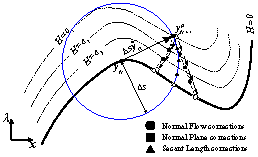
\includegraphics[scale=2.5]{FIG47.pdf}
	\caption{Two correction algorithms: Normal Flow and Normal Plane.}
	\label{fig:FIG47}
\end{figure}

Intermediate Normal Flow corrections correspond to
contours of $\bvec{H}$, $\bvec{H}_j$, where $\bvec{H}_j=\bvec{c}_{cont,j}$, 
$\Vert
\bvec{c}_{cont,j}\Vert_2>\epsilon_{tol}$, with $j$ the iteration counter. 
Normal Plane
corrections lie on a plane orthogonal to the tangent at $\bvec{y}_N$ and at
distance $\Delta s$, while Secant Length corrections are forced to lie on a
sphere of radius $\Delta s$, centered at $\bvec{y}_N$.

In any case, for the Augmented Jacobian approach,  $\bmat{B} = 
\bmat{A}^{-1}=[\bmat{DH}^T\ \ \bvec{q}_c]^{-1}$ and
$\bvec{r} = -[\bvec{H}^T\ \ V]^T$, where
$\dot{V}(\bvec{y})=\bvec{q}_c^T\dot{\bvec{y}}$.
The techniques derived from the Augmented Jacobian
approach underpin most incremental algorithms that have been developed 
for tackling stability problems in computational solid mechanics.
\cite{Wempner:1971,Riks:1972,Riks:1979,Crisfield3,Ramm:1981}. The Normal
Flow and two cases of Augmented Jacobian iterates are depicted in 
figure (\ref{fig:FIG47}), in particular the normal plane and secant length
methods. For details on the numerical linear algebra pertaining to these
methods, the interested reader can refer to the works of 
Keller\cite{Keller:1978,Keller:1983}, 
Chan and Keller\cite{ChanKeller:1982}, Griewank\cite{Griewank:1985},
Rheinboldt\cite{Rheinboldt:1983B}, Lin et.al.\cite{Lin:1987}, among others. 



\end{appendices}